\documentclass[a4paper,12pt]{article} 
\usepackage[T2A]{fontenc}			
\usepackage[utf8]{inputenc}			
\usepackage[english,russian]{babel}
\usepackage{float}
\usepackage{amsmath,amsfonts,amssymb,amsthm,mathrsfs,mathtools} 
\usepackage{cancel}
\usepackage{multirow}
\usepackage[colorlinks, linkcolor = blue]{hyperref}
\usepackage{upgreek}\usepackage[left=2cm,right=2cm,top=2cm,bottom=3cm,bindingoffset=0cm]{geometry}
\usepackage{tikz}
\usepackage{graphicx}
\usepackage{subfig}
\usepackage{titletoc}
\usepackage{pgfplots}
\usepackage{xcolor}
\usepackage{wrapfig}
\usepackage{pgfplots}
\pgfplotsset{width=10cm,compat=1.9}

\begin{document}

\begin{titlepage}
		\vspace*{\fill}
		
		\begin{center}
			
\includegraphics[scale=0.8]{MIPT.pdf}
			\\[0.7cm]\Huge Московский Физико-Технический Институт
			\\[2cm]\LARGE Отчет по эксперименту
			\\[0.5cm]\noindent\rule{\textwidth}{1pt}
			\\\Huge\textbf{Определение константы диссоциации метилового оранжевого}
			\\[-0.5cm]\noindent\rule{\textwidth}{1pt}
		\end{center}
		
		\vspace*{\fill}
		
		\begin{flushleft}
			Выполняли: \hspace{\fill} Группа:
			\\Розраенко Кирилл и Владимир Лим \hspace{\fill} Б04-202
		\end{flushleft}
	\end{titlepage}

	\setcounter{page}{2}
\section*{Цели и задачи}
Целью лабораторной работы является:
\begin{enumerate}
    \item Регистрация спектров поглощения растворов метилового оранжевого с различными
значениями pH в видимой и УФ-областях спектра;
    \item Определение рабочих длин волн для кислой и основной форм исследуемого
индикатора, нахождение изобестической точки;
    \item Проверка закона Бугера - Ламберта - Бера; определение коэффициентов экстинкции
кислой и основной форм индикатора на выбранных длинах волн;
    \item Определение константы диссоциации метилового оранжевого.
\end{enumerate}

\section*{Теоретические сведения}

\subsection*{Основные сведения спектроскопии}
Кислотно-основные индикаторы (pH-индикаторы) — органические соединения, способные изменять цвет в растворе при изменении кислотности (pH). Индикаторы широко используют в титровании в аналитической химии и биохимии. Их преимуществом является дешевизна, быстрота и наглядность 
исследования.

\begin{figure}[H]
    \centering
    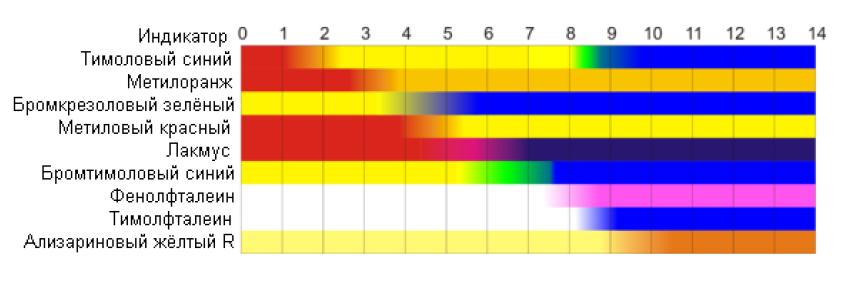
\includegraphics[scale=0.75]{Индикаторы.png}
    \centering
    \caption{Палитра различных индикаторов}
    \nonumber
\end{figure}

В основе количественных измерений в спектроскопии лежит закон Бугера - Ламберта - Бера, который связывает способность вещества поглощать свет с концентрацией данного вещества:
\begin{equation}
    \log(I_0/I) = \varepsilon_\gamma C l = D_\gamma
    \nonumber
\end{equation}

где $I$ и $I_0$ - интенсивность прошедшего и падающего на образец света; $\log$ - десятичный логарифм; $С$ - молярная концентрация; $l$ - длина оптического пути; $\varepsilon_\gamma$ - коэффициент пропорциональности, называемый молярным коэффициентом поглощения, или коэффициентом экстинкции вещества. Таким образом, оптическая плотность линейно связана с концентрацией:

\begin{equation}
    \varepsilon_\gamma C l = D_\gamma
    \nonumber
\end{equation}

Поскольку по традиции в спектроскопии длина кюветы $l$ измеряется в см, концентрация вещества - в моль/л, а оптическая плотность - безразмерная величина, то единицей измерения коэффициента экстинкции является л $\cdot$ моль / см. Величина, обратная коэффициенту экстинкции, равна толщине слоя раствора с концентрацией 1 моль/л, в котором интенсивность света уменьшается в 10 раз.

Для процесса поглощения света веществом характерна аддитивность: если в образце присутствуют несколько поглощающих форм, то оптическая плотность на данной длине волны будет определяться суммой поглощения каждой из них:

\begin{equation}
    D_\gamma = l\sum\varepsilon_i(\lambda)C_i
    \nonumber
\end{equation}

Поэтому при исследовании растворов требуется учитывать, что световой поток может поглощаться и молекулами растворителя, концентрация которых обычно на несколько порядков превышает концентрацию растворённого вещества. В итоге необходимым условием для получения спектра поглощения какого-либо вещества в растворе является полная прозрачность в данной спектральной области используемого растворителя $\varepsilon(\lambda)_s \ll \varepsilon(\lambda)_i$
Большинство часто используемых растворителей не имеют поглощения в видимой и ближней ультрафиолетовой областях спектра с границей пропускания УФ-излучения от 326 нм (бензол) до 200 нм (вода).

\subsection*{Анализ спектров мноокомпонентных систем}

Рассмотрим ситуацию, когда в растворе содержатся два вещества A и B (рис. 2) или одно вещество в двух формах (например, протонированная и депротонированная кислота HA и А-), а их концентрации связаны отношением $C_{HA} + C_{A^{-}} = C_0 = const$. В этом случае по спектру поглощения можно определить значения $С_{НА}$ и $С_{A^{-}}$. Для проведения анализа требуется, чтобы спектры этих веществ существенно отличались в некоторой области длин волн. 

\begin{figure}[H]
    \centering
    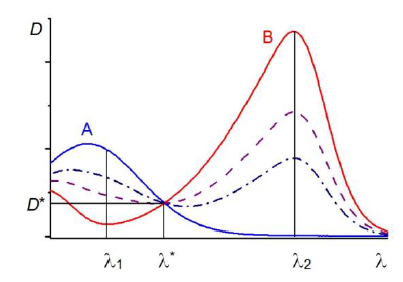
\includegraphics[scale=0.75]{Спектры.png}
    \centering
    \caption{Схема однолучевого спектрофотометра}
\end{figure}

Предположим, что в выбранной спектральной области спектры
определяемых форм вещества перекрываются незначительно. Тогда рабочую длину волны $\lambda_2$ следует выбрать так, чтобы одна форма вещества не имела на ней поглощения, а вторая поглощала возможно сильнее (правый пик на рис. 2). Зная $C_0$ и оптическую плотность $D$ на выбранной длине волны $\lambda_2$, концентрацию вещества B в растворе можно найти как:

\begin{equation}
    C_B=C_0\frac{D(\lambda_2)}{D_B(\lambda_2)}
    \nonumber
\end{equation}

где $D_B(\lambda_2)$ - оптическая плотность раствора содержащего только вещество B. Если рабочая длина $\lambda_1$ волны выбрана таким образом, что на ней поглощают обе формы, но коэффициенты экстинкции 
$\varepsilon_{HA}(\lambda_1)$ и $\varepsilon_{A^-}(\lambda_1)$ различаются, то $C_{HA}$ и $C_{A^-}$ также могут быть определены (см. далее формулу (4)).

Оптическая плотность раствора, содержащего частично диссоциированную кислоту, равна:

\begin{equation}
    D = D_{HA} + D{A^{-}} = l(\varepsilon_{HA}C_{HA} + \varepsilon_{A^-}C_{A^-})
    \nonumber
\end{equation}

Если суммарная концентрация кислоты $C_0$ поддерживается постоянной, то это выражение можно переписать в виде:

\begin{equation}
    D = lC_0(\varepsilon_{HA} + \alpha(\varepsilon_{A^-} - \varepsilon_{HA}))
\end{equation}
где $\alpha = C_{A^-}/C_0$.

Как видно из формулы (1) и рис. 2, если при некоторой длине волны $X*$ коэффициенты экстинкции обеих поглощающих форм равны между собой ($\varepsilon_A$ = $\varepsilon_B$ = $\varepsilon$*), то оптическая плотность на данной длине волны $D\lambda$* определяется только суммарной концентрацией С0 и не зависит от соотношения равновесных форм. Поэтому спектральные кривые будут пересекаться в одной точке, которую называют изобестической.
Наличие на спектрах поглощения одной или нескольких изобестических точек является хорошим критерием, позволяющим судить о наличии в растворе равновесия между двумя и только двумя веществами. Если же в серии растворов при наличии изобестической точки одна из спектральных кривых не проходит через неё, то данный раствор был приготовлен неправильно.
Точность анализа смеси растёт с увеличением разницы ($\varepsilon_A - \varepsilon_B$), достигая максимального значения в точках, где эта разница принимает наибольшее значение. Такие точки называют характеристическими.

\subsection*{Анализ кислотно0основных равновесий в растворах}

Анализ кислотно-основных равновесий в растворах является одной из важных областей приложения спектроскопии в физической химии.
Кислотой называют частицу, способную отдавать протон, а основанием - частицу, способную принимать протон. Схематически кислотно-основное равновесие может быть записано в следующем виде:

\begin{equation}
    H_xA_y \leftrightarrow H^+ + H_{x-1}A_y
    \nonumber
\end{equation}
где $H_xA_y$ - сопряжённая  кислота, $H_{x-1}A_y$ - сопряжённое основание.

Данное равновесие характеризуется константой кислотности, которая определяется произведением активностей участвующих в равновесии частиц в степенях, соответствующих стехиометрическим коэффициентам:

\begin{equation}
    K_\alpha = \frac{\alpha(H^+)\alpha(H_{x-1}A_{y^-})}{\alpha(H_xA_y)}
\end{equation}

В зависимости от рассматриваемого равновесия одна и та же частица может служить как кислотой, так и основанием. Покажем это на примере процесса диссоциации серной кислоты:

\begin{equation}
    \nonumber
    H_2SO_4 \leftrightarrow H^+ + HSO_4^-
    HSO_4^- \leftrightarrow H^+ + SO_4^{2-}
\end{equation}

В первой реакции частица $ HSO_4^-$ выступает как сопряжённое основание, во второй -
как сопряжённая кислота, а роль основания выполняет ион $SO_4^{2-}$2-. Следовательно,
кислотность частицы (способность отдавать протон) зависит не только от её собственных
свойств, но и от свойств частиц, которые принимают протон. 

Рассмотрим процесс диссоциации слабой одноосновной кислоты в водном растворе:

\begin{equation}
    HA + H_2O \leftrightarrow A^- + H_3O^+
    \nonumber
\end{equation}

Выражение для константы диссоциации записывается как:

\begin{equation}
    K_\alpha = \frac{\alpha_{A^-}\alpha_{H^+}}{\alpha_{HA}} = \frac{C_{A^-}\alpha_{H^+}}{C_{HA}}\frac{\gamma_{A^-}}{\gamma_{HA}} = \frac{\alpha C_0\alpha_{H^+})}{(1-\alpha)C_0}\gamma_{A^-}
    \nonumber
\end{equation}

\begin{equation}
    K_\alpha = \frac{\alpha}{1 - \alpha}\alpha_{H^+}\gamma_-
\end{equation}

Учтено, что в случае достаточно разбавленных водных растворов коэффициент
активности нейтральной молекулы $\gamma_{HA}$ можно положить равным единице. Коэффициент
активности $\gamma_{-}$ можно рассчитать, используя формулу Дебая - Хюккеля. Степень
диссоциации предстоит определить из спектроскопических данных.

В соответствии с формулой (1) оптическая плотность раствора является функцией от степени диссоциации кислоты и
существенно зависит от pH-среды. При добавлении сильных кислот диссоциация слабой
кислоты подавляется, а в растворе с достаточно большим pH она полностью ионизована.
Поэтому в кислом растворе можно получить спектр и определить экстинкцию не
диссоциированной кислоты $\varepsilon_{HA}$, а в щелочном растворе определить экстинкцию аниона $\varepsilon_{A^-}$. Переходная область резкого изменения степени диссоциации от $\alpha \approx 0$ до $\alpha \approx 1$ занимает 2-3 единицы pH. При меньших или больших значениях pH оптическая плотность
на рабочей длине волны будет меняться слабо, принимая значения, которые можно
обозначить соответственно как $D^{\text{кисл}}$ и $D^{\text{щел}}$:
\begin{equation}
    D^{\text{кисл}} = \varepsilon_{HA}lC_0
    \nonumber
\end{equation}
\begin{equation}
    D^{\text{щел}} = \varepsilon_{A^-}lC_0
    \nonumber
\end{equation}

В переходной области при $0 < \alpha < 1$ получаем:

\begin{equation}
    D = lC_0(\varepsilon_{HA} + \alpha(\varepsilon_{A^-} - \varepsilon_{HA})) = lC_0\varepsilon_{HA} + \alpha(lC_0\varepsilon_{A^-} - lC_0\varepsilon_{HA})
    \nonumber
\end{equation}

\begin{equation}
    D = D^{\text{кисл}} + \alpha(D^{\text{щел}} - D^{\text{кисл}})
    \nonumber
\end{equation}
откуда следует:

\begin{equation}
    \alpha = \frac{C_{A^-}}{C_0} = \frac{D - D^{\text{кисл}}}{D^{\text{щел}} - D^{\text{кисл}}}
\end{equation}

Определение константы диссоциации слабой кислоты в воде по формулам (3) И (4)
целесообразно проводить в буферных растворах с контролируемым значением pH.
Степень диссоциации находят по спектроскопическим данным, активность ионов водоро-
да определяется pH-метром, а коэффициент активности аниона кислотного остатка
рассчитывают по формуле Дебая - Хюккеля:

\begin{equation}
    \log\gamma = -\frac{0.509Z^2\sqrt{I}}{1 + \sqrt{I}}
\end{equation}

\begin{equation}
    I = \frac{1}{2}\sum C_iZ_i^2
\end{equation}
где $I$ - ионная сила раствора, $C_i$ и $Z_i$ - молярная концентрация и заряд иона. При этом
суммирование производится по всем присутствующим в растворе ионам. Обычно
концентрации реагентов, образующих буферный раствор, значительно превышают
концентрации исследуемых веществ. Поэтому ионная сила раствора на основе, например
уксусно-ацетатного буферного раствора, будет определяться преимущественно
концентрацией ацетата натрия.

Логарифмируя (3) и учитывая, что pH = $-lg\alpha_{H^+}$, получаем:

\begin{equation}
    \log K_\alpha = \log\frac{\alpha}{1 - \alpha} - pH + \log\gamma_-
\end{equation}

Эта формула позволяет рассчитывать константу диссоциации одноосновной кислоты в
буферном растворе.

\section*{Оборудование и реактивы}

0.1 М раствор $HCL$, 0.1 М растовор $NaOH$, 0.3 М раствор $CH_3COOH$, 1.0 г/л метиловый оранжевый. Мерные колбы на 50мл - 10 шт, кварцевая кювета толщиной 1 см, а также спекторфотометр.

\subsection*{Устройство спекторофотометра}

На рис. 1 показана принципиальная схема однолучевого спектрофотометра.

\begin{figure}[H]
    \centering
    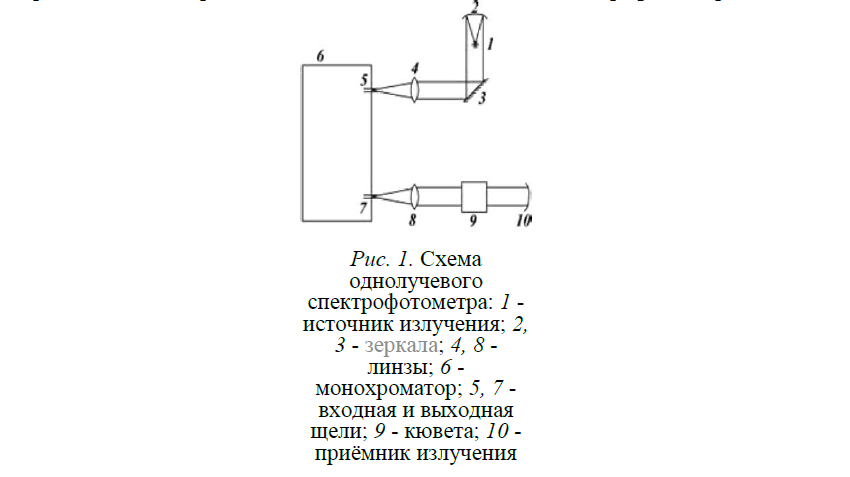
\includegraphics[scale=0.75]{Спектрофотометр.png}
    \centering
    \caption{Схема однолучевого спектрофотометра}
\end{figure}

Источником излучения в области 360-1000 нм обычно служит лампа накаливания. В качестве источника УФ-излучения в области 200-360 нм используют водородные или дейтериевые лампы. В монохроматорах в качестве диспергирующего элемента применяют призму или дифракционную решётку.

\section*{Результаты измерений и обработка результатов}

Для начала приготовим растворы как указано в методике (см. табл. 1)

\begin{table}[H]
    \begin{center}
        \begin{tabular}{|c|c|c|c|}
        \hline
            № р-ра & Р-р м-ж 0.2 г/л & Р-р К/Щ 0.1 н & Вода\\\hline
            1 & 2.0 мл & 5 мл HCl & Доб. воду в каждый р-р доводя его объем до 50 мл\\\hline
            2 & 1.5 мл & 5 мл HCl & Доб. воду в каждый р-р доводя его объем до 50 мл\\\hline
            3 & 1.0 мл & 5 мл HCl & Доб. воду в каждый р-р доводя его объем до 50 мл\\\hline
            4 & 0.5 мл & 5 мл HCl & Доб. воду в каждый р-р доводя его объем до 50 мл\\\hline
            5 & 2.5 мл & 5 мл NaOH & Доб. воду в каждый р-р доводя его объем до 50 мл\\\hline
            6 & 2.0 мл & 5 мл NaOH & Доб. воду в каждый р-р доводя его объем до 50 мл\\\hline
            7 & 1.5 мл & 5 мл NaOH & Доб. воду в каждый р-р доводя его объем до 50 мл\\\hline
            8 & 1.0 мл & 5 мл NaOH & Доб. воду в каждый р-р доводя его объем до 50 мл\\\hline
            9 & 2.0 мл & 25 мл буфер 1 & Доб. воду в каждый р-р доводя его объем до 50 мл\\\hline
            10 & 2.0 мл & 25 мл буфер 2 & Доб. воду в каждый р-р доводя его объем до 50 мл\\\hline
            11 & 2.0 мл & 25 мл буфер 3 & Доб. воду в каждый р-р доводя его объем до 50 мл\\\hline
            12 & 0 мл & 0 мл HCl & -\\\hline
        \end{tabular}
        \caption{Растворы}
    \end{center}
\end{table}

Молярная масса $\mu_{\text{метилоранжевый}}$ = 327 г/моль. Тогда $C_{\text{метилоранжевый}} = 6.1 \cdot 10^{-4}$ моль/л 

Рассмотрим спектры для данных растворов (см. рис. 4) Определим первую рабочую частоту как $\lambda_1 = 510$ нм

\begin{figure}[H]
    \centering
    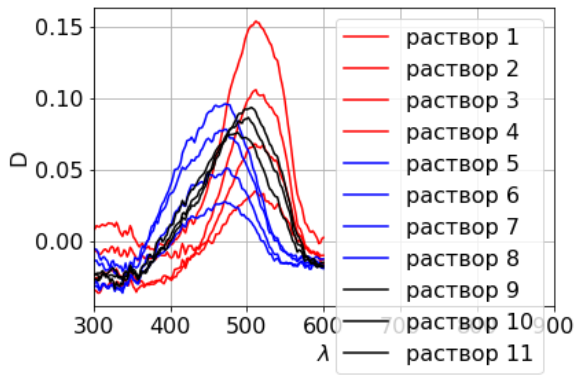
\includegraphics[scale=0.75]{Спектры растворов.png}
    \centering
    \caption{Спектры растворов}
\end{figure}

Далее построим графики зависимости оптических плотностей от концентрации индикатора для 1 - 4 раствора (см. рис. 5) и для 5 - 8 раствора (см. рис. 6)

\begin{figure}[H]
    \centering
    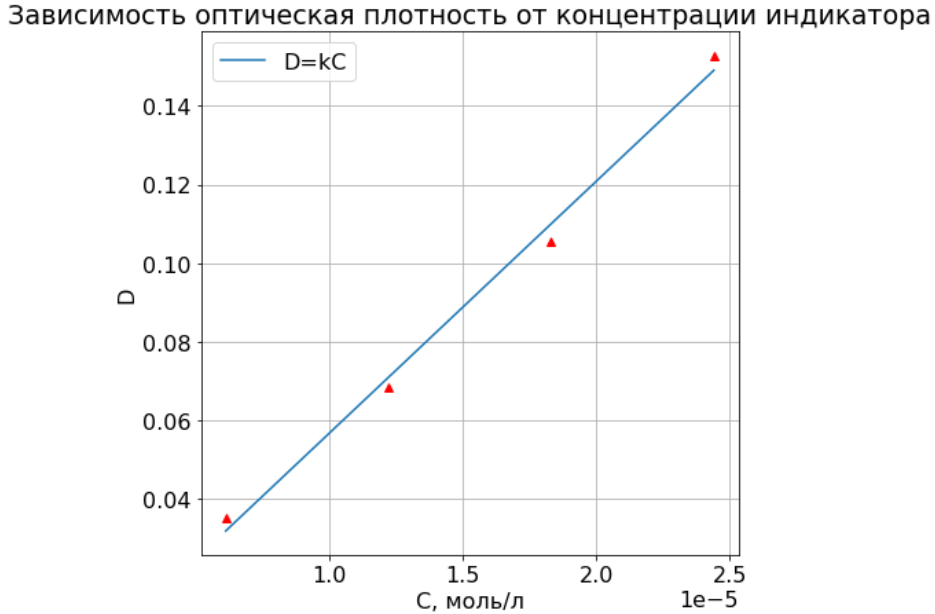
\includegraphics[scale=0.75]{1-4.png}
    \centering
    \caption{Зависимость оптической плотности от концентрации индикатора при $\lambda = 510$ нм для 1 - 4 растворов}
\end{figure}

\begin{figure}[H]
    \centering
    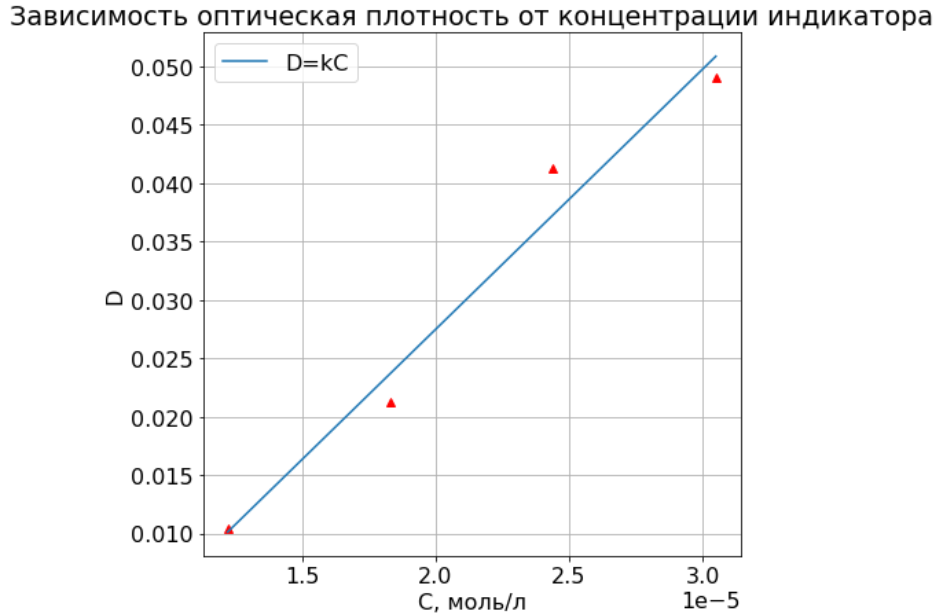
\includegraphics[scale=0.75]{5-8.png}
    \centering
    \caption{Зависимость оптической плотности от концентрации индикатора при $\lambda = 510$ нм для 5 - 8 растворов}
\end{figure}
 Тогда учитывая закон Бугера - Ламберта - Бера получаем, что $\varepsilon_{5-8}^1 = (6402 \pm 262)$ л / (моль см), $\varepsilon_{1-4}^1 = (2227 \pm 182)$ л / (моль см)

Теперь выберем другую рабочую длину воны, основываясь на спектрах $\lambda_2$ = 470 нм. Для неё соотвествующие графики (см рис. 7 и 8)

Для этой длины волны $\varepsilon_{5-8}^2 = (3669 \pm 401)$ л / (моль см) и $\varepsilon_{1-4}^2 = (3822 \pm 158)$ л / (моль см). 

\begin{figure}[H]
    \centering
    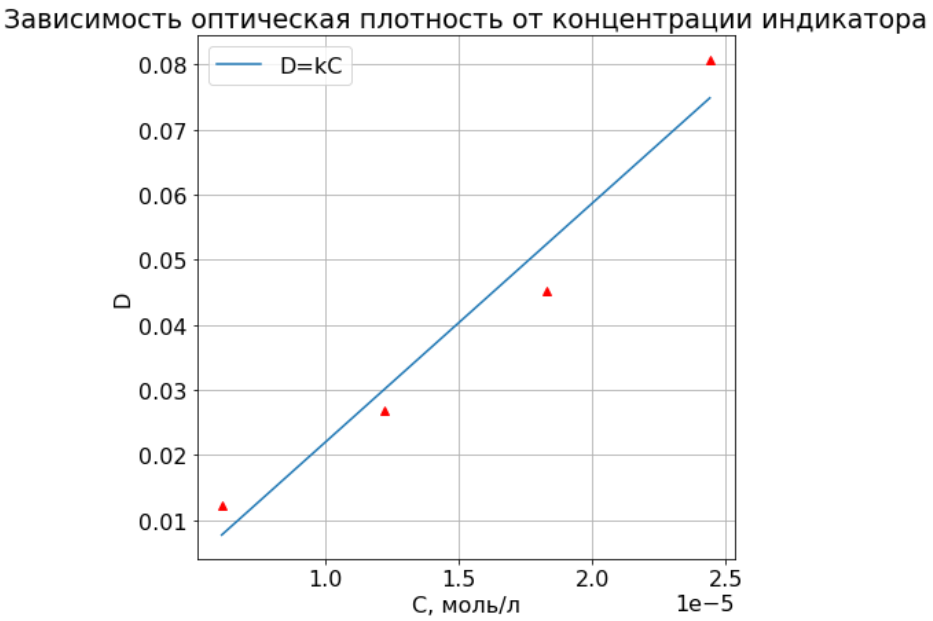
\includegraphics[scale=0.75]{1-4.2.png}
    \centering
    \caption{Зависимость оптической плотности от концентрации индикатора при $\lambda = 470$ нм для 1 - 4 растворов}
\end{figure}

\begin{figure}[H]
    \centering
    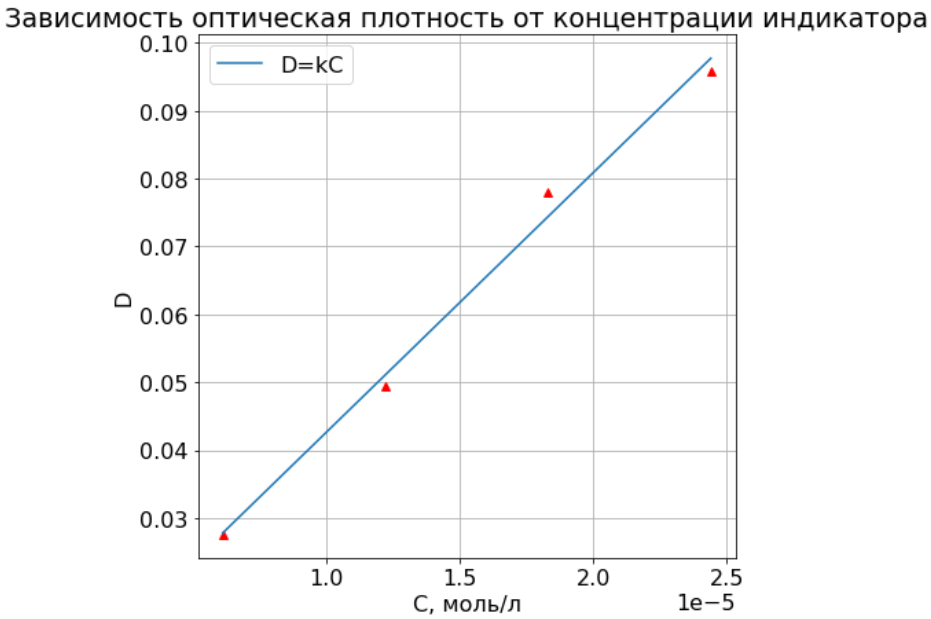
\includegraphics[scale=0.75]{5-8.2.png}
    \centering
    \caption{Зависимость оптической плотности от концентрации индикатора при $\lambda = 470$ нм для 5 - 8 растворов}
\end{figure}

Учитывая (1) найдём степень диссоциации кислоты для кажого раствора для первой длины волны и для второй соотвественно, используя выражение для степени диссоциации:

\begin{equation}
    \alpha = \frac{D - \varepsilon_{HA}lC}{lC(\varepsilon_A - \varepsilon_{HA})}
    \nonumber
\end{equation}

\begin{equation}
    \alpha = \frac{C_{A^-}}{C_0} = \frac{D - D^{\text{кисл}}}{D^{\text{щел}} - D^{\text{кисл}}}
    \nonumber
\end{equation}

Тогда для буферов степень диссоциации при первой длине волны $\alpha_1^1$ = 0.11 $\alpha_2^1$ = 0.26, $\alpha_3^1$ = 0.36. При второй длине волны $\alpha_1^2$ =0.12, $\alpha_2^2$ = 0.25     , $\alpha_3^2$ = 0.39.

Далее найдём активности по формуле Дебая - Хюккеля (5) и (6) найдём $\gamma$ = -0.046 и высчитаем константу диссоциации по (7) формуле и усредним:
\begin{equation}
    \log K_\alpha = -4.3
    \nonumber
\end{equation}
    
\begin{equation}
    K_\alpha = 10^{-4.3} = (5.0 \pm 0.1) * 10^{-5} 
    \nonumber
\end{equation}

\section*{Вывод}
В ходе работы мы:
\begin{enumerate}
    \item Успешно сняли спектры поглощения для диссоциированной и недиссоциированной форм метилового оранжевого в УФ-областях спектра.
    \item Определили рабочие длины волн для кислой и основной форм исследуемого индикатора. 
    \item Убедились в справедливости закона Бугера-Ламберта-Бера
    \item Определили константу кислотности $K_\alpha$ метилоранжа
\end{enumerate}. 

Результат, полученный нами, оказался довольно близок по порядку к табличному значению $\approx10^{-4}$. Отсюда можем заключить, что для окрашенных веществ, таких, как метилоранж, спектрофотометрия является неплохим способом для определения их свойств.

\end{document}
